\section{Question 5}

Table \ref{tbl:Q5} illustrates the rise time, overshoot and settling time for
set values of $\chi$, $\zeta$ and $\omega_0$.

\begin{table}[H]\centering
  \begin{tabular}{ccc|ccc}
  $\chi$  & $\zeta$  & $\omega_0$  & $T_r$  & $M$      & $T_s$   \\ \hline
  $0.5$   & $0.7$    & $0.1$       & $8.2$  & $14.40$   & $39.0$    \\ \hline
  $0.5$   & $0.7$    & $0.2$       & $5.0$  & $34.67$  & $23.7$  \\ \hline
  $0.5$   & $0.8$    & $0.2$       & $4.95$ & $31.72$  & $24.25$ \\ \hline
  \end{tabular}
  \caption{Rise time ($T_r$) in seconds, overshoot ($M$) as a percentage of the
    output's steady state value, and settling time $T_s$ in seconds for set
    values of $\chi$, $\zeta$ and $\omega_0$.}
  \label{tbl:Q5}
\end{table}


Due to our step response requirements, the best control performance is given by
the third set of $(\chi, \zeta, \omega_0)$ parameters. All three requirements
are fulfilled, as opposed to the case of the first set, and in comparison to the
case of the second set, the rise time and overshoot are less, while their
settling times are comparable.

Figures \ref{fig:Q5.1}, \ref{fig:Q5.2} and \ref{fig:Q5.3} depict the step
response for the three sets of $(\chi, \zeta, \omega_0)$ parameters.

\begin{figure}[H]\centering
  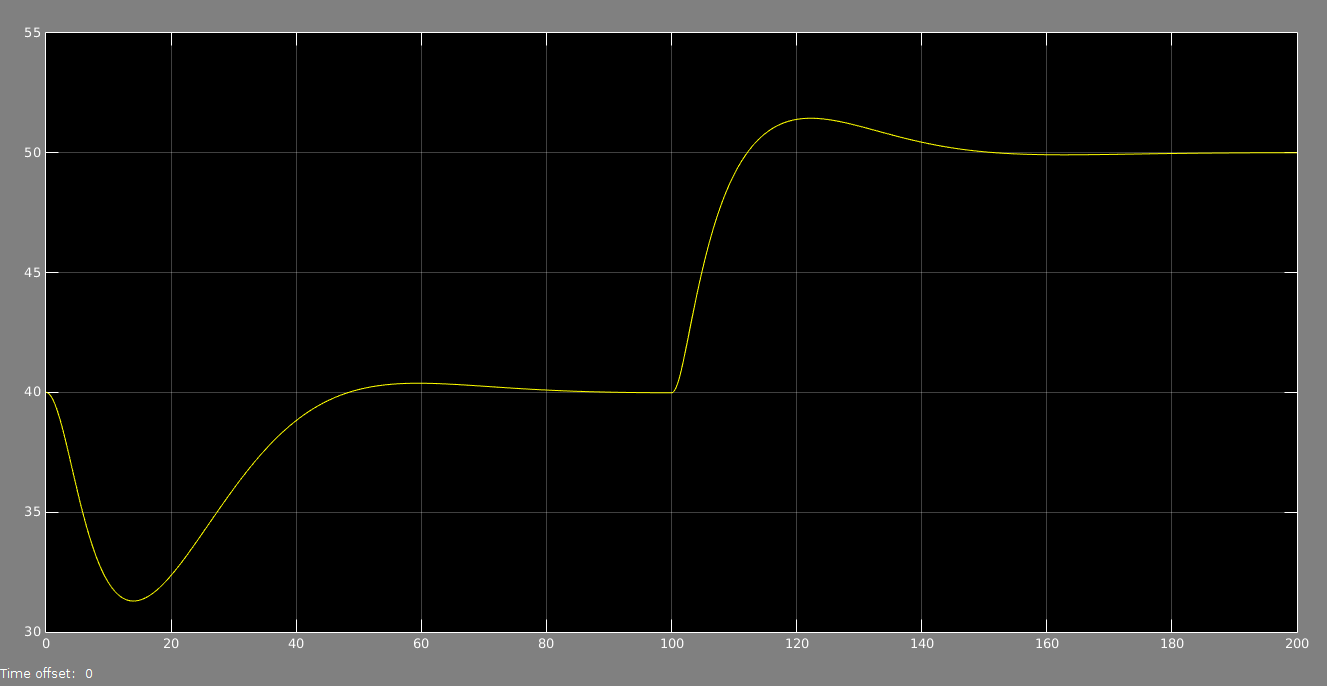
\includegraphics[scale=0.3]{./images/5/tank_2_setting_1.png}
  \caption{Step response for $(\chi, \zeta, \omega_0) \equiv (0.5, 0.7, 0.1)$.}
  \label{fig:Q5.1}
\end{figure}

\begin{figure}[H]\centering
  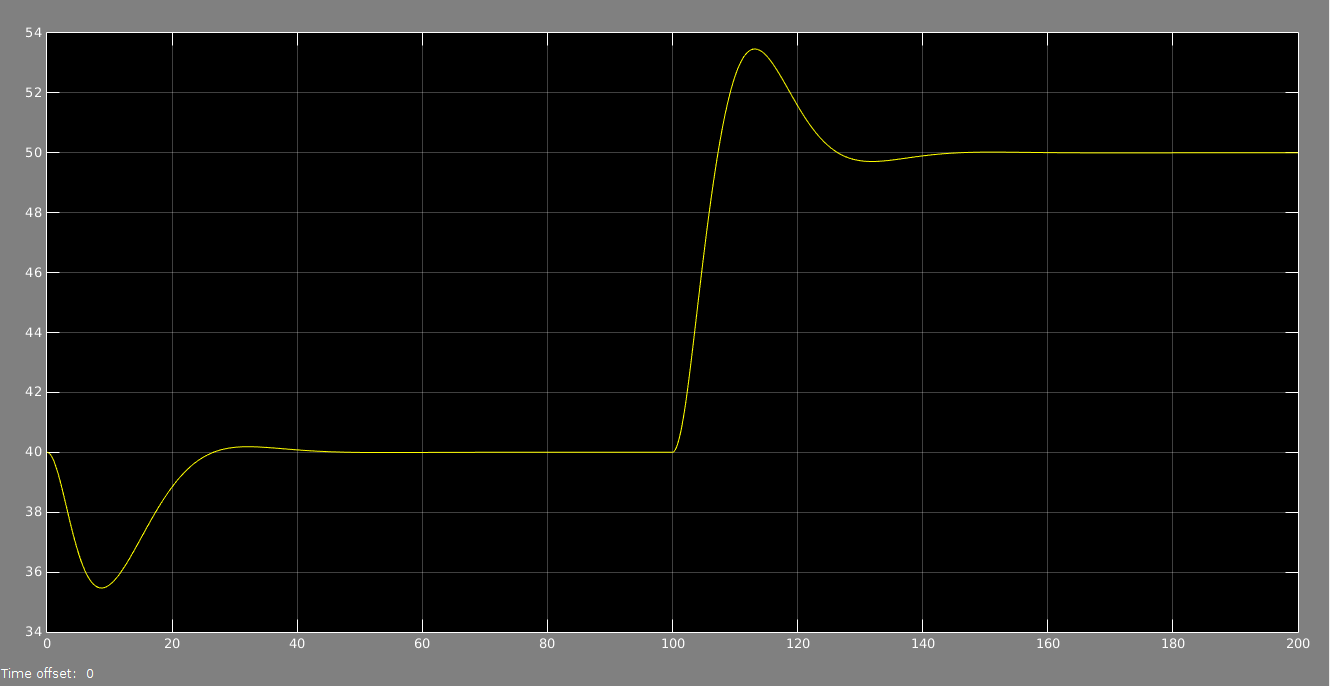
\includegraphics[scale=0.3]{./images/5/tank_2_setting_2.png}
  \caption{Step response for $(\chi, \zeta, \omega_0) \equiv (0.5, 0.7, 0.2)$.}
  \label{fig:Q5.2}
\end{figure}

\begin{figure}[H]\centering
  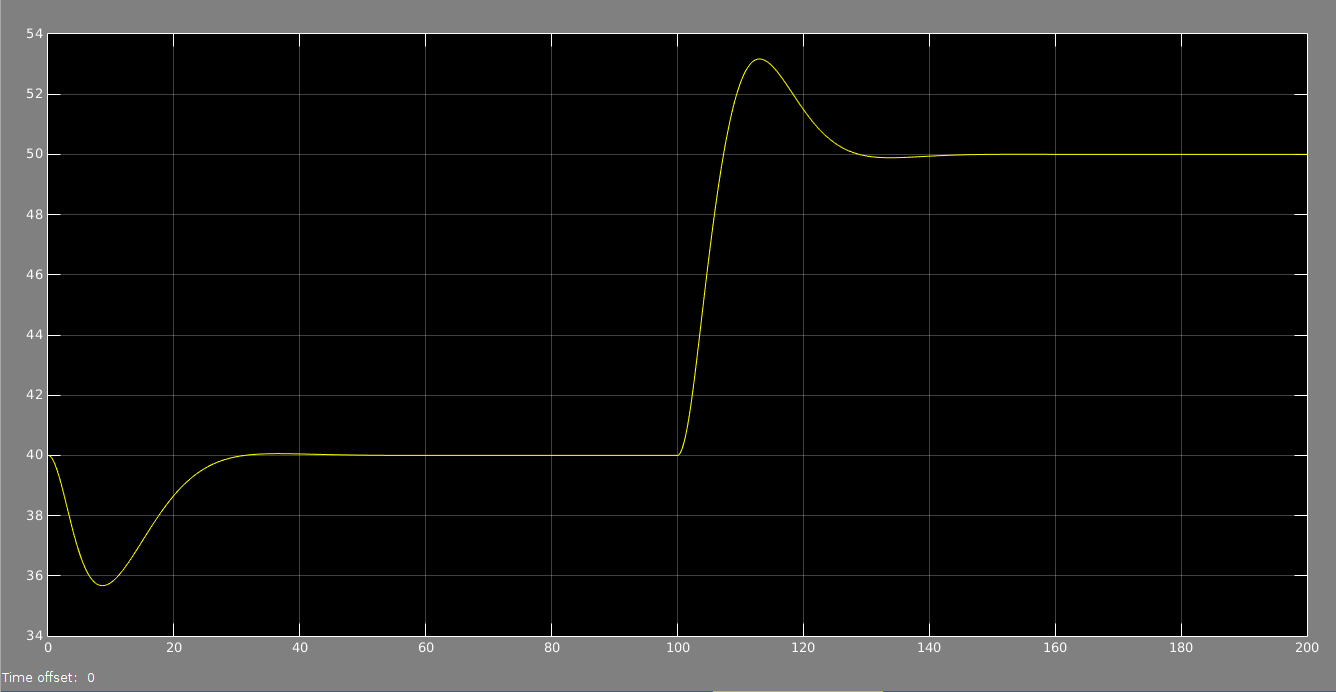
\includegraphics[scale=0.3]{./images/5/tank_2_setting_3.png}
  \caption{Step response for $(\chi, \zeta, \omega_0) \equiv (0.5, 0.8, 0.1)$.}
  \label{fig:Q5.3}
\end{figure}
